\documentclass[11pt,preprint, authoryear]{elsarticle}

\usepackage{lmodern}
%%%% My spacing
\usepackage{setspace}
\setstretch{1.2}
\DeclareMathSizes{12}{14}{10}{10}

% Wrap around which gives all figures included the [H] command, or places it "here". This can be tedious to code in Rmarkdown.
\usepackage{float}
\let\origfigure\figure
\let\endorigfigure\endfigure
\renewenvironment{figure}[1][2] {
    \expandafter\origfigure\expandafter[H]
} {
    \endorigfigure
}

\let\origtable\table
\let\endorigtable\endtable
\renewenvironment{table}[1][2] {
    \expandafter\origtable\expandafter[H]
} {
    \endorigtable
}


\usepackage{ifxetex,ifluatex}
\usepackage{fixltx2e} % provides \textsubscript
\ifnum 0\ifxetex 1\fi\ifluatex 1\fi=0 % if pdftex
  \usepackage[T1]{fontenc}
  \usepackage[utf8]{inputenc}
\else % if luatex or xelatex
  \ifxetex
    \usepackage{mathspec}
    \usepackage{xltxtra,xunicode}
  \else
    \usepackage{fontspec}
  \fi
  \defaultfontfeatures{Mapping=tex-text,Scale=MatchLowercase}
  \newcommand{\euro}{€}
\fi

\usepackage{amssymb, amsmath, amsthm, amsfonts}

\def\bibsection{\section*{References}} %%% Make "References" appear before bibliography


\usepackage[round]{natbib}

\usepackage{longtable}
\usepackage[margin=2.3cm,bottom=2cm,top=2.5cm, includefoot]{geometry}
\usepackage{fancyhdr}
\usepackage[bottom, hang, flushmargin]{footmisc}
\usepackage{graphicx}
\numberwithin{equation}{section}
\numberwithin{figure}{section}
\numberwithin{table}{section}
\setlength{\parindent}{0cm}
\setlength{\parskip}{1.3ex plus 0.5ex minus 0.3ex}
\usepackage{textcomp}
\renewcommand{\headrulewidth}{0.2pt}
\renewcommand{\footrulewidth}{0.3pt}

\usepackage{array}
\newcolumntype{x}[1]{>{\centering\arraybackslash\hspace{0pt}}p{#1}}

%%%%  Remove the "preprint submitted to" part. Don't worry about this either, it just looks better without it:
\journal{Journal of Finance}

 \def\tightlist{} % This allows for subbullets!

\usepackage{hyperref}
\hypersetup{breaklinks=true,
            bookmarks=true,
            colorlinks=true,
            citecolor=blue,
            urlcolor=blue,
            linkcolor=blue,
            pdfborder={0 0 0}}


% The following packages allow huxtable to work:
\usepackage{siunitx}
\usepackage{multirow}
\usepackage{hhline}
\usepackage{calc}
\usepackage{tabularx}
\usepackage{booktabs}
\usepackage{caption}


\newenvironment{columns}[1][]{}{}

\newenvironment{column}[1]{\begin{minipage}{#1}\ignorespaces}{%
\end{minipage}
\ifhmode\unskip\fi
\aftergroup\useignorespacesandallpars}

\def\useignorespacesandallpars#1\ignorespaces\fi{%
#1\fi\ignorespacesandallpars}

\makeatletter
\def\ignorespacesandallpars{%
  \@ifnextchar\par
    {\expandafter\ignorespacesandallpars\@gobble}%
    {}%
}
\makeatother

\newenvironment{CSLReferences}[2]{%
}

\urlstyle{same}  % don't use monospace font for urls
\setlength{\parindent}{0pt}
\setlength{\parskip}{6pt plus 2pt minus 1pt}
\setlength{\emergencystretch}{3em}  % prevent overfull lines
\setcounter{secnumdepth}{5}

%%% Use protect on footnotes to avoid problems with footnotes in titles
\let\rmarkdownfootnote\footnote%
\def\footnote{\protect\rmarkdownfootnote}
\IfFileExists{upquote.sty}{\usepackage{upquote}}{}

%%% Include extra packages specified by user

%%% Hard setting column skips for reports - this ensures greater consistency and control over the length settings in the document.
%% page layout
%% paragraphs
\setlength{\baselineskip}{12pt plus 0pt minus 0pt}
\setlength{\parskip}{12pt plus 0pt minus 0pt}
\setlength{\parindent}{0pt plus 0pt minus 0pt}
%% floats
\setlength{\floatsep}{12pt plus 0 pt minus 0pt}
\setlength{\textfloatsep}{20pt plus 0pt minus 0pt}
\setlength{\intextsep}{14pt plus 0pt minus 0pt}
\setlength{\dbltextfloatsep}{20pt plus 0pt minus 0pt}
\setlength{\dblfloatsep}{14pt plus 0pt minus 0pt}
%% maths
\setlength{\abovedisplayskip}{12pt plus 0pt minus 0pt}
\setlength{\belowdisplayskip}{12pt plus 0pt minus 0pt}
%% lists
\setlength{\topsep}{10pt plus 0pt minus 0pt}
\setlength{\partopsep}{3pt plus 0pt minus 0pt}
\setlength{\itemsep}{5pt plus 0pt minus 0pt}
\setlength{\labelsep}{8mm plus 0mm minus 0mm}
\setlength{\parsep}{\the\parskip}
\setlength{\listparindent}{\the\parindent}
%% verbatim
\setlength{\fboxsep}{5pt plus 0pt minus 0pt}



\begin{document}



\begin{frontmatter}  %

\title{Question 2}

% Set to FALSE if wanting to remove title (for submission)




\author[Add1]{Vincent Reinshagen\footnote{\textbf{Contributions:}
  \newline \emph{The authors would like to thank no institution for
  money donated to this project. Thank you sincerely.}}}
\ead{vreinshagen@outlook.de}





\address[Add1]{Stellenbosch University, Stellenbosch, South Africa}

\cortext[cor]{Corresponding author: Vincent Reinshagen\footnote{\textbf{Contributions:}
  \newline \emph{The authors would like to thank no institution for
  money donated to this project. Thank you sincerely.}}}

\begin{abstract}
\small{
I will analyze longevity and music progression
}
\end{abstract}

\vspace{1cm}





\vspace{0.5cm}

\end{frontmatter}

\setcounter{footnote}{0}



%________________________
% Header and Footers
%%%%%%%%%%%%%%%%%%%%%%%%%%%%%%%%%
\pagestyle{fancy}
\chead{}
\rhead{}
\lfoot{}
\rfoot{\footnotesize Page \thepage}
\lhead{}
%\rfoot{\footnotesize Page \thepage } % "e.g. Page 2"
\cfoot{}

%\setlength\headheight{30pt}
%%%%%%%%%%%%%%%%%%%%%%%%%%%%%%%%%
%________________________

\headsep 35pt % So that header does not go over title




\hypertarget{introduction}{%
\section{\texorpdfstring{Introduction
\label{Introduction}}{Introduction }}\label{introduction}}

The music industry is in big change. The last twenty years since the
first appearances of music streaming services, the whole business model
has been under change. TO investigate how or if the change als
influenced established bands who are already popular, I will investigate
songs of Metallica and Coldplay and set them into relation with a
Spotify dataset to compare the songs to other aritsts.

Although the data set contains song data, a hypothesis which could be
setup is that the success of a song is perfectly correlated to the
Albums popularity. If this was the case, further analyiss could be
broken down to album level which would simplify the data work
significantly. The following plot thus shows a box plot of the
popularity of songs per album.

\begin{figure}[H]

{\centering \includegraphics{Question2_files/figure-latex/Popularity by album-1} 

}

\caption{Caption Here \label{Figure1}}\label{fig:Popularity by album}
\end{figure}

We can see that the popularity of sings per album is rather spread.
Analysis on album level is therefroe not advisable.

While both bars have a long history, it is interesting if they are still
active today. The next plot shows the song releases per band over time

\begin{figure}[H]

{\centering 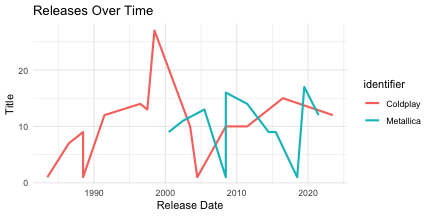
\includegraphics{Question2_files/figure-latex/Figure2-1} 

}

\caption{Caption Here \label{Figure2}}\label{fig:Figure2}
\end{figure}

The plot shows two things. The first and most important one is that
metallica misses pre 2000 data. The comparison can therefore only be
done post 2000. We can see that Coldplay released songs on a more
regular basis since 2000 than Metallica

\hypertarget{change-of-song-duration}{%
\section{\texorpdfstring{Change of song duration
\label{Meth}}{Change of song duration }}\label{change-of-song-duration}}

In recent years the hypothesis was set up that songs becam shorter over
time for two reaosns. The first one to be preferred by different
algorithms which are apparently supposed to prefer short songs and the
other reason is the rise of social media, where long songs are not
important either but only a few good seconds are important to put them
under a video. TO test if that is true and also if this applies to
Coldplay and Metallica this will be plotted below.

\begin{figure}[H]

{\centering 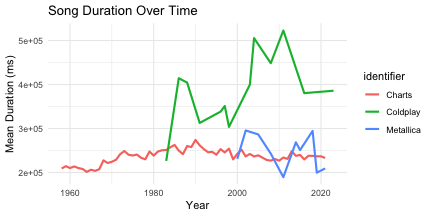
\includegraphics{Question2_files/figure-latex/Figure3-1} 

}

\caption{Caption Here \label{Figure3}}\label{fig:Figure3}
\end{figure}

We can see that since the 1990s across all spotify songs there is a
clear downwards trend for the average song length, although the sample
size is small, metallica seems to have a slightly decreasing trend too.
Coldplay on the other hand has a clear upwards trend for the song
duration

\newpage

\hypertarget{references}{%
\section*{References}\label{references}}
\addcontentsline{toc}{section}{References}

\hypertarget{refs}{}
\begin{CSLReferences}{0}{0}
\end{CSLReferences}

\hypertarget{appendix}{%
\section*{Appendix}\label{appendix}}
\addcontentsline{toc}{section}{Appendix}

\hypertarget{appendix-a}{%
\subsection*{Appendix A}\label{appendix-a}}
\addcontentsline{toc}{subsection}{Appendix A}

Some appendix information here

\hypertarget{appendix-b}{%
\subsection*{Appendix B}\label{appendix-b}}
\addcontentsline{toc}{subsection}{Appendix B}

\bibliography{Tex/ref}





\end{document}
